\startchapter{Model:  BSTS-U-MIDAS}
\label{chapter:newsol}





\section{Motivation}   

We propose a hybrid model between a partial model and a full system model for macroeconomic data forecasting. BSTS-U-MIDAS consists of two parts: a Bayesian Structural Time Series (BSTS) model, and  U-MIDAS model. The first part captures the dynamic feature of the target variable. The second part includes a large number of macroeconomic panel data as predictors. To specific, we adopt spike-and-slab regression for variable selection to handle the high dimensionality problem, and use BMA to deal with model uncertainty and instability. 

Currently, in the full system approach, the dynamic factor model is a good method for forecasting macroeconomic variables with mixed frequency data. On the other hand, in the partial model approach, MIDAS is easily implemented and is flexible enough to handle the ragged edge data problem. A combination such as a dynamic factor MIDAS is a good choice. However, the factor model has its limitation. Indeed, factors can summarize and extract useful information from predictors; however, factors may extract noise too \cite{Bai2009}. Choosing factors based on the  ordering of the eigenvalues does not guarantee that we get factors with high predictability. Evidence shows that model averaging outperforms modeling based on factors \cite{Ouysse2013}. If most macroeconomic variables are highly correlated, a few selected variables are able to capture the important information just like factors can do. Research shows that forecasts from variables are highly correlated with the forecasts from factors \cite{Bai2009}. Moreover, with the factors as predictors,a forecasting model is less useful for interpreting the relationship between macroeconomic variables that we are interested in. We choose spike-and-slab regression and BMA to deal with parameter proliferation instead of a factor model.  


We adopt U-MIDAS instead of regular MIDAS because we do not want to impose arbitrary restrictions on the parameters. Since we introduce spike and slab regression and BMA in the model, the weighting scheme for handling the parameter proliferation problem is not necessary. An U-MIDAS model is good enough for addressing the ragged edge data problem. In our model, the BSTS component  deals only with the dynamics of the target variable since we only focus on forecast performance and in such way BSTS has less computational burden. In our model, in order to avoid spurious regression, all predictors are filtered by detrending, deseasonalization, and scaling, which is done by using 'forecast' package in R \cite{Hyndman2015}. 


Our contribution is that we are the first to combine BSTS and MIDAS for macroeconomic nowcasting. We also adopt a vertically aligned method \cite{Altissimo2010} to include leading variables into the MIDAS model directly. This method is very flexible and easy to implement, and the only disadvantage is that it needs to recalculate the model every time when a new variable comes out.


\section{Model Specification}

The stages involved in specifying the model are as follows:
\textbf{Bayesian Structural Time Series} 

\begin{itemize}
	\item {Use Kalman filter to whiten time series;}
	\item {Control for trend and auto-aggression;}
	\item {Build a model for the predictable part of time series.}
\end{itemize}



\noindent \textbf{Spike and slab regression} for variable selection 

\begin{itemize}
	\item {Find regressors that predict the target.}
\end{itemize}

\noindent \textbf{Bayesian model averaging} for final forecast.

\begin{itemize}
	\item {Find forecasts across many possible forecast models.}
\end{itemize}



The first part of our model is a structural time series model(STM). \citeA{Harvey2006}  reviews  structural time series models for forecasting. Structural time series models decompose time series into different stochastic components like trend, seasonality, and cycle. The flexible structure allows the models  to handle irregular data such as missing data and mixed frequency data. The flexibility also makes forecasting and nowcasting more feasible.     

According to Harvey, the STM approach is different from the Box-Jenkins ARIMA approach which dominated the 1970's and 1980's time series forecasting \cite{Harvey2006, Frale2011}. An ARIMA model can be represented in state-space form. With the development of computing power and new algorithms, the STM has been given more attention due to its good forecasting performance.


\subsection{Local linear trend model with regression}

\citeA{Harvey1990a}, \citeA{Durbin2012}, \citeA{Petris2008} and many others have advocated the use of the Kalman filter for time series forecasting.


In our model, we only include three components: trend, autoregression and regression components. According to our experiment, detrended and deseasonalized predictors and a deseasonalized target variable have better forecast performance. Since our goal is  forecasting, we don't include seasonal terms in our model, but it can be done within our model \cite{Scott2014b}. 


The ``basic structural model" decomposes the time series into four components: a level, a local trend, seasonal effects and an error term. In contrast to the Box-Jenkins ARIMA approach, STM is able to handle some irregular data such as being nonstationary, heterosedastic, nonlinear, and non-Gaussian. The Kalman filter is used to formulate the likelihood function and conduct inference.\\


\textbf{Local linear trend model with regression}


\begin{itemize}
	\item {Observation equation(level + regression): $$y_t = \mu_t + z_t + v_{t}, \quad v_{t} \sim N(0, V)$$}
	
	\item {State equation 1 (random walk + trend): $$\mu_t = \mu_{t-1} + b_{t-1} + w_{1t}, \quad w_{1t} \sim N(0, W_{1})$$}
	
	\item {State equation 2 (random walk for trend): $$b_t = b_{t-1} + w_{2t}, \quad w_{2t} \sim N(0, W_{2})$$}
	
	
	\item {Regression component: $$z_t = \beta x_t ,$$ By appending a constant $1$ ot state vector $\alpha$ and appending $\beta x_t$ to observation matrix $F$, we only increase the dimension of the state vector $\alpha$ by one~\cite{Scott2014a}.} 
	
\end{itemize}



\begin{itemize}
	\item {Parameters to estimate: $$\theta: \beta, V, W_{1}, W_{2}$$}
	\item {States to estimate: $$\alpha:  \mu_t, b_t $$}
\end{itemize}




The Kalman filter and is used to estimate the parameters and states. Those estimations are used to forecast in the Kalman filter framework.\\




\textbf{Optimal Kalman forecast}: 	
		
$$\hat y_t =  \mu_t + z_t + K_t ( \hat y_{t-1} - y_{t-1} )$$


where $K$ is optimal Kalman gain which is a function of the variance terms $v_{1t},w_{1t}, w_{2t}$. In general, the optimal forecast will be a weighted average of past observations and the current observation. The weight $K$ depends on variances of the error terms (See Appendix A for detail) .\\ 


\textbf{Advantages of the Kalman filter}:

The Kalman filter has several advantages. First of all, it has no problem with mixed frequency. Second, it has no problem with unit roots or other kinds of non-stationarity as well. Since it does not require stationary data, it does not need a differencing or identification stage, so it is easy to automate. Third, it has a nice Bayesian interpretation. It updates its estimates when new observation arrives. Fourth, it has good forecast performance. It decomposes time series into several stochastic processes which are able to capture the dynamics of the time series.   




\textbf{Disadvantages of the Kalman filter}: 

The Kalman filter model assumes linearity, and is based upon noise terms that are normally distributed. This strong assumption is not always met in practice. Furthermore, the computational complexity increases linearly in the number of observations and quadratically in the size of the model. This is the reason why we prefer  model only the dynamics of the target variable by the Kalman filter and only take regression component $z_t = \beta x_t$ as one state.





\subsection{MIDAS for mixed frequency data}

Though the Kalman filter can handle the mixed frequency data problem and therefore the ragged edge data problem, it becomes computationally difficult when  high dimensionality presents itself in the state vectors.  We tried to model a dynamic regression component in our model. It models the dynamics of the predictors by setting the $\beta's$ of the predictors as the states in the state-space specification, but this did not improve the forecast accuracy. Since our goal is to forecast, and not to fit the model,  we adopt the MIDAS model to handle the mixed frequency problem. MIDAS includes the high-frequency data directly in the model, which simplifies the computation and improves the efficiency. We choose U-MIDAS since it does not impose restrictions on the parameters by weighting schemes. We adopt a flexible and easy way to align the ragged edge data which is similar to \citeA{Altissimo2010}. 

We realign each  high frequency time series in the sample to match the low frequency target variable according to the  forecast horizon  vertically. For example, to match a quarterly target variable from a daily predictor $y_{q+h}$, ($q$ is the quarter and $h$ is the forecast horizon), we realign all of the predictors to the current date to form a balanced data set. For daily data, the alignment is as follows:

$$\tilde x_{i, q} = x_{i, q + k_{i}} \, ,$$

where $k_{i}$ is number of days of the publication lags or leads for $i$th variable. For financial data, the number of trading days in one month is 22, so we have $k = {0, ...,22 \times 3}$. Since we focus on nowcast, we tend to choose those variables with leads. Specifically, GDP publication lag usually is two months, so for a daily data, we may have $k \in {0, ...,22 \times 2}$ leads, and for  monthly data, we may have $k = {0, ..., 3 \times 2}$. 

The $\tilde x_{i, q}$ is skip-sampled data; for example, if $k$ is 25, to match up quarterly GDP data, the $\tilde x_{i, q}$ is the 25th daily observation in the each quarter. Applying this method to each predictor, we get a balanced dataset $\tilde X_q$. 

Here is a example of an alignment of quarterly and monthly data when we want to forecast second quarter target variable but we only have monthly data up to May.

\begin{center}
Vertical alignment:		$\begin{bmatrix}
	y_{2nd \, quarter}  &  & \,\,\,\quad ;& y_{1st \, quarter} & &; ...\\
	x_{May} & x_{Apr} & x_{Mar}; &  x_{Feb} & x_{Jan} & x_{Dec} ;...
	\end{bmatrix}$
	
	$\begin{bmatrix}	
	
	y_{2nd \, quarter} & |  & x_{May} & x_{Apr} & x_{Mar} \\
	y_{1st \, quarter} & |  & x_{Feb} & x_{Jan} & x_{Dec} \\
	... & |  & ... & ... & ...	
	\end{bmatrix}$\\
\end{center} 

The main advantages of this approach is its simplicity. Whenever new data come out, we can reestimate the model and update forecasts. 

The disadvantage is every time when new data come out, the balanced dataset $\tilde X_q$ changes, the correlations between variables change, and the stability of model may change as well \cite{Foroni2013} .



\section{Variable Selection: Spike-and-Slab Regression}

In the Bayesian framework, the \textit{spike and slab prior} is an effective variable selection device to achieve sparsity \cite{George1997, Madigan1994a}  . It has been used in macroeconomic forecasting \cite{Rodriguez2010,Kaufmann2012,Ferrara2014} .


\begin{figure}[h]
\centering
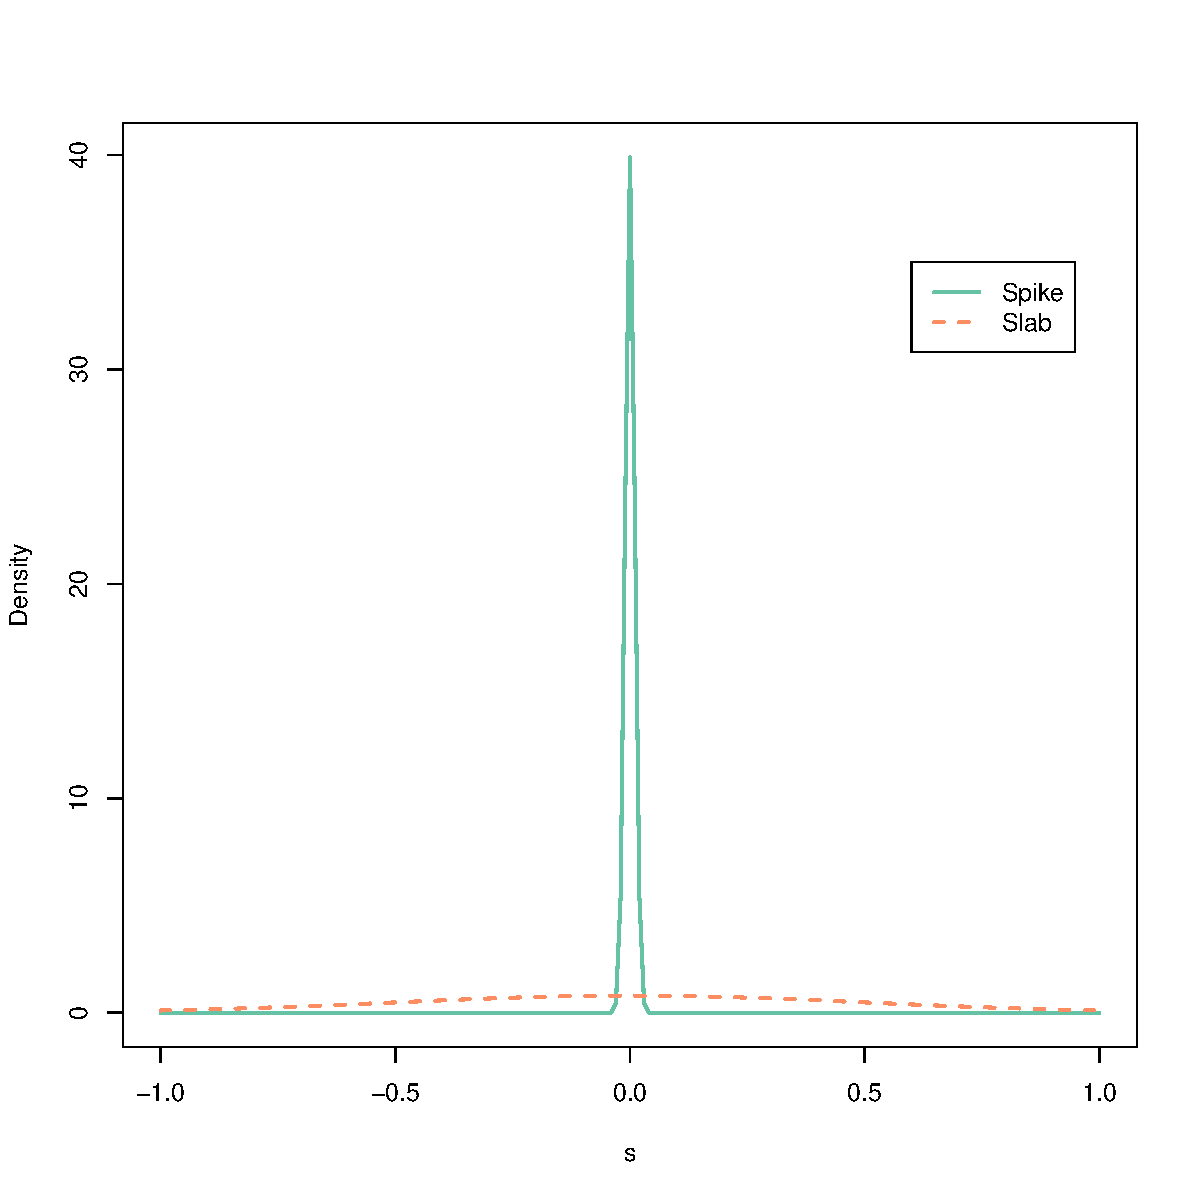
\includegraphics[width=0.5\linewidth]{Figures/spike}
\caption{Spike and slab prior}
\label{fig:spike}
\end{figure}


If there are $N$ predictors, then there are at least $2^N$ possible linear models in the model space. The spike-and-slab prior is a way to carry out the variable selection. One of the approaches is a stochastic search variable selection strategy (SVSS), which takes the prior to be a mixture of two normal distributions:

$$\beta_i \sim \gamma_i N(b_i,\varphi^2)   + (1-\gamma_i) N(0, c \varphi^2)$$

where $\gamma$ is a vector of indicator variable. The marginal distribution $p(\gamma)$ is the ``spike" since it has positive probability mass at zero. When $\gamma_i = 1$, variable $x_i$ has a non-zero coefficient in regression. $c$ is a very small positive number, so when $\gamma_i = 0$, variable $\beta_i$ could be 'safely' estimated by zero and excluded from the regression. $\gamma_i$ is a binary random variable which can be modeled by a product of independent Bernoulli distribution.

$$\gamma_i \sim \pi_{i}^{\gamma_i}(1- \pi_{i})^{1-\gamma_i}$$

and we have:



$$\gamma \sim \prod_{i} \pi_{i}^{\gamma_i}(1- \pi_{i})^{1-\gamma_i} \, .$$


 
Given  $p(\gamma)$, a spike-and-slab prior can be factored as:  


$$ p(\beta, \sigma^{-2},\gamma) = p(\beta \mid \gamma, \sigma^{-2})p(\sigma^{-2} \mid \gamma )p(\gamma)  \,  ,$$


where $\pi_i$ is predictor $x_i$'s probability of inclusion in the regression.  When detailed prior information is unavailable, it is convenient to set all $\pi_i$ equal to the same number, $\pi$. The common informative prior inclusion probability can easily be elicited from the expected number of nonzero coefficients. For example, if $n$ out of $N$ coefficients are expected to be nonzero, then we can set $\pi = n/N$ in the prior. For the expected number of predictors $n$, we choose 4 in our model since in a cross validation, the performance of model with 4 is better than performances of models with other numbers.

In such a hierarchical structure, a variable $x_i$ with $\gamma_i = 1$ has a \textit{conditionally conjugate} ``slab" prior: 


$$ \beta_{\gamma} \mid \sigma^{2} ,\gamma  \sim N(b_{\gamma}, \sigma^{2}(\Omega_{\gamma}^{-1})^{-1}) \,  ,$$


$$\frac {1}{\sigma^{2}} \mid \gamma \sim  \Gamma(\frac{df}{2}, \frac{ss}{2})  \,  .$$


where $b_{\gamma}$ is a vector of prior guesses for the regression coefficients, $\sigma^{2}$ is the overall variance level of error, and $\Omega^{-1}$ is a prior precision matrix, and  $\Omega_{\gamma}^{-1}$  is rows and columns of  $\Omega^{-1}$ when $\gamma_i = 1$.


Conventionally,  $b_{\gamma}$ is set to equal $0$, and $\Omega^{-1} \propto X^T X$, which  is known as Zellner's informative g-prior \cite{Chipman2001}.  If we have specific information about $b_{\gamma}$, a informative prior will helpful for the estimation. The matrix $X^T X$ is the total Fisher information matrix in the full data, and we can  parametrize $\Omega^{-1} = \kappa (X^T X)/T$, which representing the average information available from $\kappa$ observations. And it means we places $\kappa$ observations worth of weight on the prior mean $b_{\gamma}$ \cite{Scott2014a}. 







It shows that given $\gamma$,  the prior for the precision follows a Gamma distribution with parameters $\frac{df}{2}$ and $\frac{ss}{2}$. Thus, the reciprocal of the mean of the Gamma distribution $ss/df$ is a prior estimate of $\sigma^2$. 

The ``Slab" prior is a very weakly informative prior which is close to being flat. In some sense,  $ss$ can be interpreted as a prior sum of squared error, and the $df$ can be interpreted as a prior sample size. The bigger the sample size is , the more information about the parameters we have, and then  we have a better precision and a smaller variance for estimation of the parameters. Further details of elicitation of the priors are discussed in~\cref{sec:prior}.

It turns out that there is a connection between SSVS and LASSO \cite{Yuan2005}. A spike and slab prior for $\beta_i$ can be formulated as follows:

$$ \beta_i = (1-\gamma_i) \delta(0) + \gamma_i DE(0, \lambda ) $$

$\delta(0)$ is the point mass distribution centered at zero for predictors which is excluded in model. $DE(0, \lambda )$ is the double exponential (Laplace) distribution with density $\lambda e^{−\lambda |x|}$ which is for the predictors which is included in model.

The prior for indicator $\gamma$ is 
$$p(\lambda)  \propto \pi^{|\gamma|}(1-\pi)^{p-|\gamma|} |X_{\gamma}^T X_{\gamma}|^{\frac{1}{2}}  .$$

$|\gamma| = \sum_{i=1}^{p} \gamma_i $ is the number of predictors in the model. $|X_{\gamma}^T X_{\gamma}|^{\frac{1}{2}}$ penalizes models with correlated predictors. It can be shown that the posterior mode of $\gamma$ selects the same parameters as the LASSO. 

\section{Model Estimation Using MCMC}
 

We follow  \citeA{Scott2014a}  and implement  Markov Chain Monte Carlo (MCMC) to obtain the posterior distribution of the coefficients. For a MCMC process, we need to know the full set of conditional distributions of the parameters. \citeA{Scott2014a}  give a detailed algorithm and `bsts' package in R to implement the algorithm \cite{Scott2015}. 



\subsubsection{The conditional posterior of $\beta$ and $\sigma^2$ given $\gamma$}






Suppose we have a local linear trend model, the observation equation is  



$$y_t = \mu_t + \beta \mathbf{x}_t + v_{t}$$  




We subtract the target time series component $\mu$ from $y_t$, and get an axillary variable $y^* = y_t - \mu_t$.  Then we have  


$$y_t^* = y_t - \mu_t = \beta x_t + \epsilon_t \sim N(\beta x_t, \sigma^2)$$


And we are left with a standard spike-and-slab regression. We can use ``stochastic search variable selection"(SSVS) algorithm to draw from $p(\beta_{\gamma}, \sigma^2 | \gamma, \alpha, \mathbf{y}^*)$, where vector $\mathbf{y}^* = y_{1:T}^*$ is all the information about $y^*$ up to time $T$.   





Then conditional on $\gamma$, the joint posterior distribution for $\beta$ and $\sigma^2$ can be estimated from standard conjugacy formula \cite{Gelman2013} :   







$$\beta_{\gamma} \mid \sigma, \gamma, \mathbf{y}^*  \sim  N(b_{\gamma}, \sigma^2(V_{\gamma}^{-1}))$$  






$$\frac {1}{\sigma^{2}} \mid \gamma, \mathbf{y}^* \sim  \Gamma(\frac{df+T}{2}, \frac{ss + \tilde{S}}{2})$$  




More discussion can be found in \citeA{Scott2014b} and   \citeA{Ferrara2014}. The details are discussed in~\cref{sec:mcmc}.



\subsubsection{The marginal posterior of $\gamma$}



Due to the conjugacy, we can get analytical expression for the marginal posterior of $\gamma$ by marginalizing over  $\beta_{\gamma}$ and ${1}/{\sigma^{2}}$:




$$\gamma \mid \mathbf{y}^* \sim C(\mathbf{y}^*) \frac{|\Omega^{-1}|^{1/2}}{|V_{\gamma}^{-1}|^{1/2}} \frac{p(\gamma)}{SS_{\gamma}^{\frac{T}{2} -1}} \, ,$$




where $C(\mathbf{y}^*)$ is a normalizing constant. 



\subsubsection{MCMC process}






Since we have a  state-space model and a spike-and-slab regression, the parameters we need to  estimate are as follows: 







\textit{Parameters to estimate}: $$\theta_1: 	V_{1t}, W_{1t}, W_{2t}$$ and $$\theta_2: \beta, \sigma^2,  \gamma$$







\textit{States to estimate}: $$\alpha:  \mu_t, b_t$$





Since the state $\alpha$ has Markov property, we assume that conditional on state $\alpha$, the time series components which relate to $v_{1t},w_{1t},w_{2t}$, and the regression components related to $\beta, \gamma$ are independent. Then we can follow three steps as follows:


1. Simulate the state $\alpha$ from 


$$\alpha \sim p(\alpha \mid \mathbf{y}, \theta_1, \theta_2) \, .$$


2. Simulate the parameters for the time series components:


$$\theta_1 \sim  p(\theta_1  \mid \mathbf{y},\alpha,  \theta_2) \, .$$


3. Simulate the parameters for the regression components:

$$\theta_2 \sim  p(\theta_1  \mid \mathbf{y},\alpha,  \theta_1) \, . $$




Iterating the three steps, we can get the posterior distribution of state $\alpha$ and parameters $\theta_1, \theta_2$ given $\mathbf{y}$. Under a Gaussianity assumption, the $p(\alpha|y)$ is solved by a stochastic version of the Kalman smoother \cite{Durbin2002}. The first set of parameters $\theta_1$ are obtained via conjugacy prior. For the variance parameters $ W_{t}, W_{2t}$, they have  independent inverse Gamma priors, and their full conditional posterior distributions are independent inverse Gamma distributions as well. The second set of parameters $\theta_2$ can be estimated by the stochastic search variable selection (SSVS) algorithm from \citeA{George1997}, which uses a Gibbs sampling algorithm.  Further details are discussed in~\cref{sec:mcmc}.

One of issues of Bayesian variable selection is computational difficulty. It can be shown that the some form of the joint posterior of parameters may have more than one mode \cite{Park2008}. The multiple modality could cause conceptual and computational problems. Conceptually, it is hard to summarize the posterior distribution. Computationally, the Gibbs sampler will have difficulty to converge or stuck at one corner and not explore the entire model space enough. There are many methods developed to tackle these issues\cite{Ishwaran2005}. We are aware these issues, and try to increase the number of iteration to improve the estimation.



\section{Bayesian Model Averaging}







Let $\phi$ be $\alpha, \theta_1, \theta_2$, then with the draw of state and parameters from their posterior distribution, we can get the posterior predictive distribution for the target variable $y$:  



$$p(\tilde y \mid \mathbf{y}) = \int p(\tilde y \mid \phi)p(\phi \mid \mathbf{y})~d \phi \, .$$



For each draw of $\phi^{(i)}$ from $p(\phi \mid \mathbf{y})$, we can sample a $\tilde y$ from $p(\tilde y \mid \phi)$. The sample of draws from the posterior predictive distribution $p(\tilde y \mid \mathbf{y})$ can give us the information that we need for forecasting. To summarize the information, we can use the mean, median, or mode as a point forecast of the target variable $y$.

To consider the model uncertainty, we also can get a forecast interval or  use a histogram or density to summarize the forecast. To understand the impact of the predictors on th target variable, we can get the inclusion probability of specific predictors by summary of $\gamma_k$. For example, we can take the average over draws of $\gamma$ to see which predictors have high probability of being in the regression. 



%\input chapters/3/sec_latexhelp